\documentclass[10pt]{beamer}
\usetheme{metropolis}
\usecolortheme{default}
\usepackage{booktabs}
\usepackage{amsmath}
\usepackage{graphicx}
\usepackage{tikz}
\usetikzlibrary{arrows.meta, positioning}


\title{The Paradox of Voting}
\subtitle{ECO1028 --- Why Do Rational People Vote?}
\author{Beatriz Gietner\\
\texttt{beatriz.gietner@dcu.ie}}

\begin{document}

\maketitle

\begin{frame}{Outline}
\tableofcontents
\end{frame}

\section{Introduction \& Prerequisites}

\begin{frame}{The Central Puzzle: The Rationality Gap}
\href{https://www.jstor.org/stable/pdf/30023729.pdf}{\alert{\textbf{Schumpeter (1942):} The "Primitive" Voter}}


\begin{quote}
"...the typical citizen drops down to a lower level of mental performance as soon as he enters the political field. He argues and analyzes in a way which he would readily recognize as infantile within the sphere of his real interests. He becomes a primitive again."
\end{quote}


\textbf{The "Psychic Economy" of Politics:}
\begin{itemize}
\item Political questions feel like "fictitious" leisure-hour interests
\item Not like a "business proposition" - dangers seem far off
\item \alert{Citizens expend less disciplined effort on mastering a political problem than on a game of bridge}
\end{itemize}


\alert{Think about it:} Why might you spend weeks researching a €1,000 phone but only 10 minutes researching a candidate who manages billions in taxes?
\end{frame}

\begin{frame}{What You Need to Know}
\textbf{Four prerequisite pillars:}
\begin{enumerate}
\item \textbf{Cost-Benefit Analysis}
\begin{itemize}
\item People weigh costs against benefits before acting
\item Opportunity cost: voting time = time not spent elsewhere
\end{itemize}

\item \textbf{Probability \& Pivotality}
\begin{itemize}
\item Your vote only matters if it changes the outcome
\item 10-person lunch vote vs. 150M-person election
\end{itemize}

\item \textbf{Information Costs}
\begin{itemize}
\item Learning about politics takes time and mental effort
\item Return on investment problem
\end{itemize}

\item \textbf{Winner-Take-All Systems}
\begin{itemize}
\item 50.1\% wins everything, 49.9\% wins nothing
\item First-Past-The-Post amplifies the paradox
\end{itemize}
\end{enumerate}
\end{frame}

\begin{frame}{Diagnostic Check}
\textbf{Test your understanding:}


\textbf{Question 1:} €100 buried in a 10-acre field. Takes 5 hours to find. Do you dig?
\begin{itemize}
\item Tests: Cost-benefit logic
\end{itemize}


\textbf{Question 2:} Why do people buy lottery tickets when expected value is negative?
\begin{itemize}
\item Tests: Expressive utility vs. instrumental utility
\end{itemize}


\textbf{Question 3:} Can you name a US Presidential election decided by exactly one vote?
\begin{itemize}
\item \alert{Spoiler:} There hasn't been one
\item In electorate of 100M: $P \approx 0.00006$ (six in 100,000)
\item Your vote is more likely to be decisive if you flip a coin 14 times and get all heads ($1/2^{14} \approx 0.000061$)
\end{itemize}
\end{frame}


\section{Historical Development}

\begin{frame}{Intellectual Precursors}
\textbf{Knut Wicksell (1896):}
\begin{itemize}
\item "Just taxation" and unanimity rules
\item How can we design political institutions that get voluntary agreement?
\end{itemize}


\textbf{Duncan Black (1948):}
\begin{itemize}
\item Group decision-making theory
\item Developed the median voter theorem
\end{itemize}


\textbf{Kenneth Arrow (1951):}
\begin{itemize}
\item Impossibility theorem: No perfect voting system
\item Nobel Prize 1972
\end{itemize}


But none of these directly addressed \emph{why} people vote
\end{frame}

\begin{frame}{The Breakthrough: Downs (1957)}
\textbf{Anthony Downs, \emph{An Economic Theory of Democracy}}


\textbf{Key innovation:}
\begin{itemize}
\item Applied economic reasoning to political behaviour
\item Parties = firms competing for votes
\item Voters = consumers maximizing utility
\end{itemize}


\textbf{The rational voter model:}
\begin{itemize}
\item Voters calculate expected utilities from each candidate
\item Vote for candidate promising highest expected utility
\item But immediately recognized the paradox: $P$ is tiny
\end{itemize}


Downs \emph{identified} the paradox but didn't fully resolve it
\end{frame}

\begin{frame}{The Golden Age: 1960s--1980s}
\textbf{Mancur Olson (1965):} \emph{The Logic of Collective Action}
\begin{itemize}
\item Why small groups organize and large groups free-ride
\item Voting as collective action problem
\end{itemize}


\textbf{Gordon Tullock (1967):}
\begin{itemize}
\item First formal analysis of the paradox
\item Introduced the psychic income term (negative cost)
\end{itemize}

\href{https://www.cambridge.org/core/journals/american-political-science-review/article/theory-of-the-calculus-of-voting/500608E51991E92AC96EB6860F1192CA}{\textbf{Riker \& Ordeshook (A Theory of the Calculus of Voting, 1968):}}

\begin{itemize}
\item Formalized the $R = PB + D - C$ equation
\item First major empirical test using survey data
\item Found $D$ (civic duty) dominates
\end{itemize}
\end{frame}

\begin{frame}{Continued Development: 1970s--1990s}
\textbf{Ferejohn \& Fiorina (The paradox of not voting, 1974; Closeness counts, 1975):}
\begin{itemize}
\item Minimax regret strategy
\item "Rescuing rational choice theorists from this embarrassing predicament"
\end{itemize}

\textbf{Fiorina (The voting decision, 1976):}
\begin{itemize}
\item Expressive voting hypothesis
\item Voting as consumption, not investment
\end{itemize}


\textbf{Ashenfelter \& Kelley (Determinants of participation, 1975):}
\begin{itemize}
\item Large-scale empirical study (1,893 voters) $\rightarrow$ Confirmed importance of $D$ and $C$
\end{itemize}


\textbf{1980s--1990s:}
\begin{itemize}
\item Aggregate data studies (Foster 1984, Patterson \& Caldeira 1983)
\item International comparisons (Jackman, 1987)
\end{itemize}
\end{frame}

\begin{frame}{Modern Developments: 2000s--Present}
\textbf{Experimental evidence:}
\begin{itemize}
\item DellaVigna et al. (2017): Social image concerns
\item Gerber et al. (2008): Social pressure effects
\item Blais \& Young (1999): Habit vs. rational calculation
\end{itemize}


\textbf{New theoretical approaches:}
\begin{itemize}
\item behavioural economics integration
\item Evolutionary explanations
\item Group-based voting models
\end{itemize}


\textbf{Current state:}
\begin{itemize}
\item No consensus solution
\item Multiple explanations coexist
\item Focus shifted to: \emph{When} do different motivations dominate?
\end{itemize}
\end{frame}

\begin{frame}{Celebrity Political Endorsements}
\begin{columns}[T]
\begin{column}{0.40\textwidth}
\centering
\includegraphics[width=\textwidth]{pic2topic1.JPG}

\small Taylor Swift endorsing Joe Biden in 2020
\end{column}



\begin{column}{0.48\textwidth}
\centering
\includegraphics[width=\textwidth]{pic1topic1.JPG}

\small Zohran Mamdani's social media advocacy
\end{column}
\end{columns}

\vspace{0.5cm}

\alert{Question:} How does social media change the expressive benefits of voting?
\end{frame}

\begin{frame}{Social Media \& the Amplification of Expressive Benefits}
\textbf{How social media has changed the calculus:}

\begin{itemize}
\item \textbf{The "I Voted" sticker phenomenon - "clout farming"}
\begin{itemize}
\item Voting becomes a public performance, not a private act
\item Instagram/TikTok posts broadcasting political participation
\item Massively increases the \alert{audience} for your expressive signal
\end{itemize}

\item \textbf{Celebrity political endorsements}
\begin{itemize}
\item Taylor Swift endorsing Democratic candidates
\item Zohran Mamdani's social media advocacy
\item Influencers making voting "cool" or socially desirable
\end{itemize}

\item \textbf{Impact on the $D$ term:}
\begin{itemize}
\item Social media \alert{amplifies} psychic benefits of civic duty
\item Increases social pressure ("Did you vote?")
\item Makes abstention more costly (social shame)
\item DellaVigna et al. (2017): People vote to signal to others
\end{itemize}
\end{itemize}


\alert{Modern twist:} $D$ might now include \emph{social media signaling value}
\end{frame}

\section{The Rational Voter Model}

\begin{frame}{The Two-Phase Voting Process}
\textbf{Voting isn't a single calculation, but a two-step process:}

   
\begin{enumerate}
\item \textbf{Phase 1: The Evaluation Phase (The "Who")}
\begin{itemize}
\item Comparing candidates to determine which outcome is better.
\item \textbf{Output:} The Utility Differential ($B$).
\end{itemize}

   
\item \textbf{Phase 2: The Participation Phase (The "Whether")}
\begin{itemize}
\item Deciding if the benefit of voting justifies the personal cost.
\item \textbf{Output:} The decision to vote or abstain ($R$).
\end{itemize}
\end{enumerate}

   
\alert{The Paradox of Voting exists entirely within Phase 2.}
\end{frame}

\begin{frame}{Key Variables}
\textbf{Notation used throughout:}
\begin{itemize}
\item $P$ = Probability your vote is \alert{pivotal} (decisive)
\item $p$ = Expected fraction of votes for your preferred candidate ($0 \le p \le 1$)
\item $B$ = Benefit differential between candidates
\item $C$ = Cost of voting
\item $D$ = Civic duty / psychic benefit
\item $N$ = Total number of voters
\end{itemize}
\end{frame}

\begin{frame}{Phase 1: The Evaluation Phase}
\textbf{Goal: Determine which candidate promises the most utility.}


The voter envisages the "streams of utility" derived from policies promised by each candidate.

   
\textbf{The Calculation of $B$:}
\[ B = E(U_i | P_{a\text{ wins}}) - E(U_i | P_{b\text{ wins}}) \]

   
\begin{itemize}
\item If $B > 0$, the voter prefers Candidate a.
\item If $B < 0$, the voter prefers Candidate b.
\item If $B = 0$, the voter is indifferent.
\end{itemize}


\footnotesize{Note: $B$ is a measure of the \emph{stakes} of the election for that individual.}
\end{frame}

\begin{frame}{Phase 2: The Participation Phase}
\textbf{Goal: Determine if casting a ballot is a rational investment.}

Once a preference ($B$) is established, the voter evaluates the act of voting as a purely instrumental act.

\begin{center}
\Large
\alert{$R = (P \times B) - C$}
\end{center}

\centering
where $R$ = net return from voting


\textbf{Individual $i$ votes if and only if $R > 0$}


\footnotesize{This model assumes the only purpose of voting is to influence the outcome.}
\end{frame}

\begin{frame}{Breaking Down $R = PB - C$}
\begin{description}
\item[$P$] = Probability your vote is decisive (Pivotality) 
\begin{itemize}
\item The chance your vote breaks or creates a tie.
\end{itemize}


\item[$B$] = Utility benefit from your preferred candidate winning
\begin{itemize}
\item Calculated in Phase 1; represents the differential utility streams.
\end{itemize}


\item[$C$] = Cost of voting
\begin{itemize}
\item Time, effort, opportunity cost, or even mildly bad weather.
\end{itemize}
\end{description}


\centering
\textbf{Expected benefit of voting} = $PB - C$
\end{frame}

\begin{frame}{Calculating $P$: The Ball-Drawing Model}
\textbf{Your vote matters only in two specific scenarios:}
\begin{itemize}
\item \textbf{Scenario 1 (Breaking a tie):} All other votes are exactly tied. Your vote is the decider (weighted at $100\%$).
\item \textbf{Scenario 2 (Creating a tie):} Your preferred candidate loses by one vote. Your vote forces a draw (weighted at $50\%$ because it leads to a $50/50$ chance of eventually winning).
\end{itemize}

\vspace{0.4cm}
\textbf{The Logic (Mueller, Section 14.1.1):}
\begin{itemize}
\item Think of each voter as drawing a ball from a bag.
\item Fraction $p$ are labeled "Candidate 1" and $(1-p)$ are labeled "Candidate 2".
\item For odd $N$, the probability $P$ of being instrumental is:
\end{itemize}

\begin{equation*}
P = \frac{3e^{-2(N-1)(p-\frac{1}{2})^2}}{2\sqrt{2\pi(N-1)}}
\end{equation*}
\end{frame}

\begin{frame}{Understanding the Formula: Key Assumptions}
\textbf{What does the model assume?}

\begin{enumerate}
\item \textbf{Independence:} Each voter votes independently
\begin{itemize}
\item No coordination, no social pressure
\item Questionable assumption (families, social networks)
\end{itemize}

\item \textbf{Knowledge of $p$:} You have beliefs about the vote share
\begin{itemize}
\item From pre-election polls, media coverage, historical data
\item But polls have sampling error!
\end{itemize}

\item \textbf{Large $N$:} Normal approximation works
\begin{itemize}
\item Valid for national elections
\item Less valid for small local elections
\end{itemize}
\end{enumerate}

\alert{Key insight:} The formula tells us what $P$ \emph{would be} given your beliefs about $p$, not what $P$ actually is.
\end{frame}

\begin{frame}{What Does This Formula Tell Us?}
$$P = \frac{3e^{-2(N-1)(p-\frac{1}{2})^2}}{2\sqrt{2\pi(N-1)}}$$

\textbf{Key insights:}
\begin{enumerate}
\item $P$ falls \alert{exponentially} as $N$ increases
\item $P$ falls \alert{exponentially} as $p$ diverges from 0.5
\item Even in best case ($p = 0.5$, 100M voters): $P = 0.00006$
\end{enumerate}

\textbf{The Reality:} $B$ must be roughly 16,000 times greater than $C$ for a rational vote to make sense.

\begin{alertblock}{The "p Problem"}
But how do voters know $p$ on election day? They don't! Even polls have error. This is a fundamental weakness of the model that we'll revisit later.
\end{alertblock}
\end{frame}

\begin{frame}{How Sensitive is $P$ to Changes in $p$?}
\textbf{Example: 100 million voters}

\begin{table}
\centering
\begin{tabular}{cc}
\toprule
\textbf{Vote Split ($p$)} & \textbf{Probability $P$} \\
\midrule
50-50 ($p = 0.50$) & 0.00006 (6 in 100,000) \\
51-49 ($p = 0.51$) & 0.000006 (6 in 1,000,000) \\
52-48 ($p = 0.52$) & $\approx$ 0 (essentially zero) \\
60-40 ($p = 0.60$) & $\approx$ 0 (completely negligible) \\
\bottomrule
\end{tabular}
\end{table}

\textbf{Key takeaway:} even slight movements away from 50-50 make $P$ plummet. Only in \alert{historically close} elections does $P$ have any non-negligible value - and even then it's tiny!

\footnotesize{This is why Ashenfelter \& Kelley's finding is important: the difference between thinking an election is close vs. a landslide is enormous for perceived $P$.}
\end{frame}

\begin{frame}{The Paradox Revealed}
\begin{alertblock}{If $P \approx 0$ and $C > 0$, then:}
\centering
\Large
$(P \times B) - C < 0$
\end{alertblock}


\textbf{Logical conclusion of Phase 2:}
\begin{itemize}
\item No rational, self-interested person should ever vote.
\item Cost of voting ($C$) always exceeds the instrumental expected benefit ($PB$).
\end{itemize}


\begin{exampleblock}{}
\centering
\textbf{But millions of people DO vote. Why?}
\end{exampleblock}


This is the paradox of voting.
\end{frame}

\begin{frame}{Mueller's Critical Assessment}
\textbf{Three sophisticated "fixes" to save rational choice:}


\begin{table}
\centering
\footnotesize
\begin{tabular}{p{2.5cm}p{3.5cm}p{3.5cm}}
\toprule
\textbf{Strategy} & \textbf{Logic} & \textbf{Mueller's Critique} \\
\midrule
Taste for Voting ($D$) & People vote to satisfy a "civic itch" (psychic gains) & Makes theory tautological; robs it of predictive power \\
\midrule
Game of Cat \& Mouse & If all stay home, one vote wins & With large electorates, still need large $D$ \\
\midrule
Minimax-Regret & Minimize maximum regret & Implies bizarre behaviour; inconsistent with other domains \\
\bottomrule
\end{tabular}
\end{table}


\textbf{Common problem:} each "works" but at the cost of making the theory unfalsifiable or requiring auxiliary assumptions
\end{frame}

\subsection{Solution 1: Modifying the Calculus}

\begin{frame}{Solution 1a: A Taste for Voting}
\textbf{Riker \& Ordeshook (1968): Add a "$D$" term}


\begin{center}
\Large
\alert{$R = PB + D - C$}
\end{center}


\textbf{$D$ = Psychic benefit from act of voting itself:}
\begin{itemize}
\item Civic duty, patriotic feeling, sense of participation
\item "Complying with the ethic of voting"
\item Affirming allegiance to the political system
\item NOT dependent on whether your candidate wins
\item Vote if $D - C > 0$ (since $PB \approx 0$)
\end{itemize}


\textbf{This works!} But at what cost to theory?
\end{frame}

\begin{frame}{The Epicycle Problem}
\begin{alertblock}{The problem with adding $D$}
This is a bit of a fudge. Any hypothesis can fit any data if you add enough auxiliary assumptions.
\end{alertblock}


\textbf{Example from physics:}
\begin{itemize}
\item Ptolemaic astronomy: Earth at center, planets orbit in circles
\item Observations didn't fit? Add "epicycles" - circles on circles
\item Could fit any observation, but had no predictive power
\end{itemize}


\textbf{Same problem here:}
\begin{itemize}
\item If civic duty explains voting, what else might it explain?
\item Does civic duty guide candidate choice too?
\item When does self-interest override civic duty?
\item Without a theory of $D$, we've just \emph{named} the problem
\end{itemize}
\end{frame}

\begin{frame}{Solution 1b: Voting as a Game}
\textbf{If everyone reasons that voting is irrational...}
\begin{itemize}
\item Then no one would vote
\item But then \emph{any} voter could determine the outcome!
\item So whether it's rational to abstain depends on others' decisions
\end{itemize}


\textbf{Game-theoretic approach (Ledyard 1981, Palfrey \& Rosenthal 1983):}
\begin{itemize}
\item Model as $n$-person noncooperative game (rational players act in their self-interest)
\item Each person's strategy depends on expectations about others
\item Under some assumptions, equilibria exist with positive turnout
\end{itemize}


\textbf{But:}
\begin{itemize}
\item With large electorates and uncertain costs
\item Rational individual votes only if psychic benefits exceed costs
\item \alert{We're back to needing large $D$}
\end{itemize}
\end{frame}

\begin{frame}{Solution 1c: Minimax Regret}
\textbf{Ferejohn \& Fiorina (1974):} Different decision rule


Instead of weighing events by probability:
\begin{itemize}
\item Give all events \emph{equal weight}
\item Calculate "regret" for each strategy/state combination
\item Regret = loss from choosing this strategy vs. best alternative
\item Choose strategy that minimizes maximum regret
\end{itemize}


\textbf{Key insight:}
\begin{itemize}
\item Under this rule, only $B$ is important, not $P$
\item Probability becomes irrelevant to the decision
\item Extremely conservative: avoid worst-case scenario at all costs
\end{itemize}
\end{frame}

\begin{frame}{The Minimax Regret Matrix}
\textbf{Regret for each strategy/state combination:}


\begin{table}
\centering
\begin{tabular}{l|cc}
\toprule
\textbf{Strategy} & $S_I$ (Vote Irrelevant) & $S_D$ (Vote Decisive) \\
\midrule
Vote & $C$ & $0$ \\
Abstain & $0$ & $B - C$ \\
\bottomrule
\end{tabular}
\end{table}


\textbf{Reading the table:}
\begin{itemize}
\item If I vote and my vote doesn't matter, I regret wasting $C$
\item If I abstain and my vote would have mattered, I regret losing $B-C$
\end{itemize}


\textbf{If $B \geq 2C$:} Maximum regret from abstaining = $B - C$ $>$ $C$

$\Rightarrow$ Minimax strategy: \alert{VOTE}
\end{frame}

\begin{frame}{Problems with Minimax Regret I}
\textbf{Leads to bizarre predictions:}


\textbf{Example 1:} I'm indifferent between Democrats \& Republicans
\begin{itemize}
\item $B \approx 0$, so minimax says: abstain
\end{itemize}


\textbf{But} a Nazi Party enters the race:
\begin{itemize}
\item Now $B$ (difference between Dem/Rep and Nazi) is huge
\item Minimax says: must vote to avoid tiny chance Nazi wins by one vote!
\item Even though probability is infinitesimal
\end{itemize}


\alert{This is absurd:} Entry of irrelevant third candidate forces me to vote
\end{frame}

\begin{frame}{Problems with Minimax Regret II}
\textbf{People don't act this way elsewhere:}


\begin{itemize}
\item Do you buy volcano insurance?
\item Do you buy meteorite insurance?
\item Most don't buy flood insurance even when subsidized below actuarial value
\item Losing home is at least as bad as getting wrong president
\end{itemize}


\textbf{Inconsistency:}
\begin{itemize}
\item Risk-taking with home and possessions
\item But minimax-conservative when voting?
\end{itemize}


\textbf{Without a theory of \emph{when} people use minimax regret:}
\begin{itemize}
\item We can rationalize \emph{ex post} but not predict \emph{ex ante}
\item Same problem as with $D$ term
\end{itemize}
\end{frame}

\begin{frame}{Solution 1d: Group Mobilization Models}
\textbf{Feddersen (2004)}

\begin{itemize}
\item \textbf{Logic:} Voting isn't an individual act; 
  it is a \textbf{collective action} coordinated by leaders.
\item \textbf{The "Follow the Leader" Model:}
\begin{itemize}
\item Leaders (parties, unions, churches) identify pivotal groups.
\item They use social pressure or mobilization to overcome 
  the $C$ term for the whole group.
\end{itemize}
\item \textbf{The result:} Participation is rational because 
  the group (not the individual) is pivotal.
\end{itemize}

\footnotesize{Reference: \href{https://pubs.aeaweb.org/doi/pdf/10.1257/089533004773563458}{\alert{Feddersen (2004), "Rational Choice Theory and the Paradox of Not Voting," \emph{Journal of Economic Perspectives}}}}
\end{frame}

\subsection{Solution 2: Expressive Voting}

\begin{frame}{Solution 2: Expressive Voting}
\textbf{Fiorina (1976):} Voting as expression

Voting provides utility from the act itself:
\begin{itemize}
\item You gain satisfaction from expressing your political identity
\item Similar to cheering at a sporting event
\item The value comes from participating and showing support
\item Voting becomes an act of consumption - you enjoy doing it
\end{itemize}


\textbf{Implication:} People vote because the act itself feels rewarding, independent of whether their vote changes the outcome.
\end{frame}

\begin{frame}{Two Interpretations of Expressive Voting}
\begin{enumerate}
\item \textbf{Express support for preferred candidate}
\begin{itemize}
\item Thank candidate for standing up for your interests
\item Makes $D = D' + B$ where:
\begin{itemize}
\item $D'$ = civic duty satisfaction
\item $B$ = expressive benefit from supporting preferred candidate
\end{itemize}
\item Explains \emph{why} you vote, not necessarily \emph{how}
\end{itemize}



\item \textbf{Express views about public interest}
\begin{itemize}
\item Low $P$ frees you to vote differently than if vote mattered
\item Could be more "irresponsible" or more "noble"
\end{itemize}
\end{enumerate}
\end{frame}


\begin{frame}{The Irresponsible Voter Hypothesis}
\textbf{Brennan \& Buchanan (1984):}


If voters know their vote doesn't matter:
\begin{itemize}
\item They may express preferences they'd never act on if decisive
\item Example: "Candidate X would ruin the country"
\item "But X is the only one speaking out against immigrants"
\item If you think X has no chance: vote for X to vent anxiety
\item You'd \emph{never} vote for X if your vote was decisive
\end{itemize}


\textbf{The noble voter hypothesis:}
\begin{itemize}
\item Low $P$ could also free voters to be more ethical
\item Vote for "what's good for the country" instead of self-interest
\item Express moral commitments without cost
\end{itemize}


Which dominates? Evidence is mixed.
\end{frame}


\begin{frame}{Expressive Voting: Symbolic \& "Dark Urges"}
\textbf{Mueller (Section 14.4): Not all expression is noble.}

\begin{itemize}
\item \textbf{Symbolic Attitudes:} Research shows that "symbolic attitudes" like racial or sexist prejudice often drive choice more than self-interest.
\item \textbf{Loss of Reality:} Because the voter knows their vote won't change the outcome, they feel free to vent "dark urges" or infantile impulses.
\item \textbf{The Result:} Low pivotality ($P$) decouples the voter from the real-world consequences of their choice, leading to potential polarization.
\end{itemize}


\alert{Schumpeter's Link:} This is why the citizen "drops down to a lower level of mental performance" in politics.
\end{frame}

\begin{frame}{Evidence Against Pure Expressive Voting (1)}
\textbf{Strategic voting:}
\begin{itemize}
\item People \emph{don't} vote for candidates running third or fourth
\item Don't want to "waste" their vote
\item This suggests they think votes \emph{do} matter
\end{itemize}



\textbf{Cox (1997) on tactical voting:}
\begin{itemize}
\item \textbf{Single-member districts} = districts that elect only 1 representative (e.g., US House, UK Parliament)
\item Uses First-Past-The-Post: single-winner voting rule $\rightarrow$ whoever gets most votes wins
\item Voters desert hopeless candidates and vote for "lesser evil" among top two viable options
\end{itemize}
\end{frame}

\begin{frame}{Evidence Against Pure Expressive Voting (2)}
\textbf{Example of tactical voting:}
\begin{itemize}
\item You prefer Green candidate
\item Polls show only Labour vs. Conservative are competitive
\item You vote Labour (your 2nd choice) to block Conservative from winning
\item This is \emph{strategic voting} based on viability rather than pure expression
\end{itemize}



\alert{Why this contradicts expressive voting:} If voting were purely about expressing your views, you'd vote Green regardless of whether they can win.



\textbf{Experimental evidence (Carter \& Guerette 1992, Fischer 1996):}
\begin{itemize}
\item Weak evidence that people become more altruistic when $P$ falls
\item But many subjects vote selfishly regardless of $P$
\item Suggests multiple motivations coexist
\end{itemize}
\end{frame}

\begin{frame}{Expressive vs. Ethical: What's the Difference?}
\textbf{These are often confused but conceptually distinct:}

\begin{table}
\centering
\footnotesize
\begin{tabular}{p{4cm}p{5cm}}
\toprule
\textbf{Expressive Voting} & \textbf{Ethical Voting} \\
\midrule
Explains \emph{why} you vote & Explains \emph{how} you vote \\
\midrule
Utility from act itself (like cheering) & Utility from outcomes for others \\
\midrule
Can be selfish or altruistic & Always includes others' welfare \\
\midrule
$D = D' + B$ in one interpretation & $O_i = U_i + \theta \sum U_j$ \\
& \footnotesize{($U_i$ = your utility, $\theta$ = altruism weight, $\sum U_j$ = others' welfare)} \\
\midrule
Low $P$ frees you to vote differently & High $\theta$ makes you vote for public good \\
\bottomrule
\end{tabular}
\end{table}
\end{frame}

\begin{frame}{Expressive vs. Ethical: What's the Difference?}
\textbf{Example of ethical voting:}
\begin{itemize}
\item Wealthy voter with high $\theta$ (altruism weight) votes for higher taxes on the rich
\item Personally loses money ($U_i$ decreases), but society benefits ($\sum U_j$ increases)
\item Overall satisfaction $O_i$ can still be positive if $\theta$ is large enough
\end{itemize}

\textbf{Both can coexist:}
\begin{itemize}
\item You vote expressively (to participate) \emph{and} ethically (for public interest)
\end{itemize}
\end{frame}

\subsection{Solution 3: The Ethical Voter}

\begin{frame}{Solution 3: The Ethical Voter}
\textbf{Voters have two sets of preferences:}



\begin{columns}[T]
\begin{column}{0.48\textwidth}
\begin{block}{Selfish Preferences}
\footnotesize
\begin{itemize}
\item Contains only your own utility
\item Guides market behaviour (buying bread, choosing job)
\item Standard economic rational actor
\end{itemize}
\end{block}
\end{column}

\begin{column}{0.48\textwidth}
\begin{block}{Ethical Preferences}
\footnotesize
\begin{itemize}
\item Contains utilities of others
\item Guides political behaviour (voting, civic participation)
\item Jekyll \& Hyde view
\end{itemize}
\end{block}
\end{column}
\end{columns}



\textbf{Jekyll \& Hyde:} People genuinely switch between preference sets depending on context - selfish in markets, altruistic in politics.



\textbf{The problem:}
\begin{itemize}
\item When does each preference set activate?
\item Same issue as $D$ term - needs formalization
\end{itemize}
\end{frame}

\begin{frame}{Formalizing Ethical Preferences}
\textbf{Individual $i$'s objective function:}


\begin{center}
\Large
$O_i = U_i + \theta \sum_{j \neq i} U_j$
\end{center}


\textbf{Where $\theta$ (theta) measures altruism:}
\begin{itemize}
\item $\theta = 0$: Purely selfish voter
\item $\theta = 1$: Fully altruistic voter (\href{https://www.journals.uchicago.edu/doi/abs/10.1086/257678}{Harsanyi 1955})
\item $0 < \theta < 1$: Partially ethical
\end{itemize}


Now the question becomes: What determines $\theta$?
\begin{itemize}
\item Individual characteristics (education, income, age)?
\item Context (type of election, perceived stakes)?
\item Culture and institutions?
\end{itemize}
\end{frame}

\begin{frame}{Evidence on $\theta$}
\textbf{Hudson \& Jones (1994):} Survey in Bath, England
\begin{itemize}
\item Asked voters about policy preferences
\item Would policy benefit you personally?
\item Would policy be in public's interest?
\item Estimated $\theta \approx 0.66$ (1988), $\theta \approx 0.73$ (1992)
\end{itemize}


\textbf{Economic voting literature (Cross-national comparisons):}
\begin{itemize}
\item Egotropic voting: based on personal economic situation
\item Sociotropic voting: based on national economic situation
\item US, UK, France, Germany: $\theta$ between 0.5 and 1.0
\item \alert{Denmark: $\theta \approx 0.15$} (much more egotropic/selfish!)
\end{itemize}


\textbf{The comparative puzzle:}
\begin{itemize}
\item Why do Danish voters place less weight on others' welfare?
\item Is it culture? Institutions? Welfare state design?
\item This variation suggests $\theta$ isn't fixed across contexts
\end{itemize}
\end{frame}

\begin{frame}{When Do People Vote Ethically?}
\textbf{Evidence that self-interest \emph{doesn't} fully explain voting:}


\textbf{Smith (1975):} Tax equalization vote in Oregon
\begin{itemize}
\item Simple choice: raise or lower your taxes
\item 60.7\% of large gainers favoured equalization
\item But 32.7\% of large losers \emph{also} favoured it!
\item Over 40\% voted against narrow self-interest
\end{itemize}


\textbf{Gramlich \& Rubinfeld (1982):} Michigan tax limitation
\begin{itemize}
\item Transfer recipients only moderately more likely to oppose
\item 42\% of public employees voted to restrict their own budget
\end{itemize}


Substantial minorities (and sometimes majorities) vote for "public interest"
\end{frame}

\begin{frame}{Sociotropic vs. Egotropic Voting}
\textbf{Two competing models of how voters decide:}


\begin{block}{Egotropic Voting (Self-Interest)}
\begin{itemize}
\item Vote based on personal economic situation
\item "What has the government done for \emph{me}?"
\item Example: Vote against incumbent if \emph{you} lost your job
\end{itemize}
\end{block}

\begin{block}{Sociotropic Voting (Public Interest)}
\begin{itemize}
\item Vote based on national economic situation
\item "What has the government done for \emph{the country}?"
\item Example: Vote against incumbent if \emph{national} unemployment is high
\end{itemize}
\end{block}


\textbf{Empirical evidence:} Studies estimate $\theta \approx 0.5$ to 0.7
\begin{itemize}
\item Voters place substantial weight on sociotropic considerations
\item Consistent with ethical voter hypothesis
\end{itemize}

\footnotesize{Lewis-Beck (1988), Kinder \& Kiewiet (1979)}
\end{frame}

\subsection{Solution 4: Behavioural Approach}

\begin{frame}{Solution 4: Behavioural Psychology}
\textbf{Mueller's key insight: Relax rationality, keep self-interest}


\textbf{Basic principle from behavioural psychology:}
\begin{itemize}
\item Actions followed by rewards $\uparrow$ in frequency
\item Actions followed by punishment $\downarrow$ in frequency
\item This is how all animals learn
\end{itemize}


\textbf{Voting as conditioned habit:}
\begin{itemize}
\item Ethical behaviour is learned through childhood conditioning
\item Parents reward cooperative behaviour, punish selfish behaviour
\item Schools reward following rules, punish breaking them
\item Occasional reinforcement maintains behaviour in adulthood
\item \alert{Voting becomes an "unreflective and habitual act"}
\end{itemize}


\textbf{This is still selfish behaviour:}
\begin{itemize}
\item It's a conditioned response, not a conscious ethical choice
\item You vote because you've been trained to cooperate
\end{itemize}
\end{frame}

\begin{frame}{Voting as a Conditioned Habit}
\textbf{The behavioural Reinforcement Loop (Mueller, Section 14.5)}


\centering
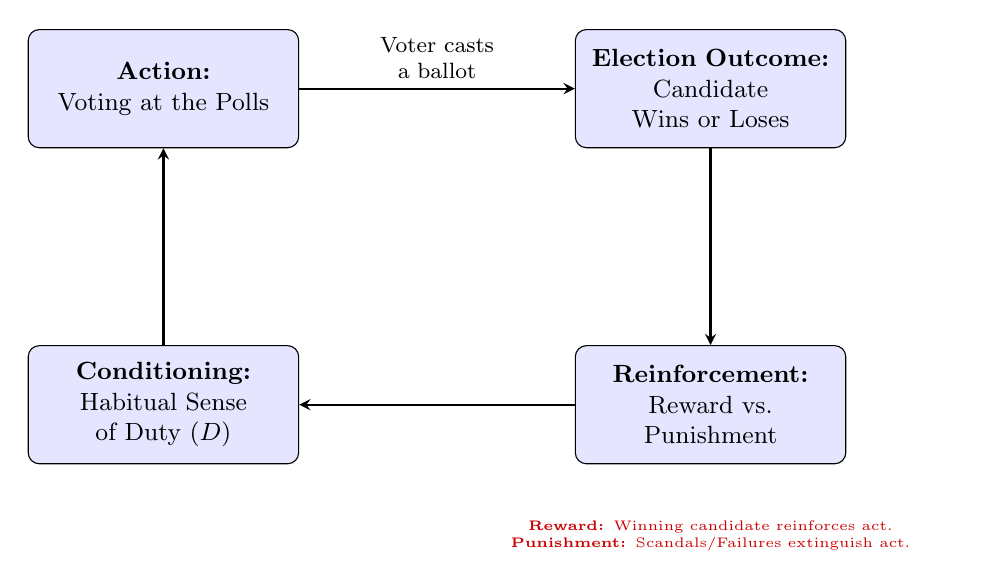
\begin{tikzpicture}[
node distance=2.5cm and 3.5cm, 
block/.style={rectangle, draw, fill=blue!10, text width=3.2cm, align=center, rounded corners, minimum height=1.5cm, font=\small},
arrow/.style={thick,->,>=stealth}
]


\node (act) [block] {\textbf{Action:}\\ Voting at the Polls};
\node (outcome) [block, right=of act] {\textbf{Election Outcome:}\\ Candidate Wins or Loses};
\node (reinforce) [block, below=of outcome] {\textbf{Reinforcement:}\\ Reward vs. Punishment};
\node (habit) [block, below=of act] {\textbf{Conditioning:}\\ Habitual Sense of Duty ($D$)};


\draw [arrow] (act) -- node[above, font=\footnotesize, text width=2cm, align=center] {Voter casts a ballot} (outcome);
\draw [arrow] (outcome) -- (reinforce);
\draw [arrow] (reinforce) -- (habit);
\draw [arrow] (habit) -- (act);


\node [below=0.6cm of reinforce, text width=6cm, align=center, font=\tiny, color=red!80!black] {
\textbf{Reward:} Winning candidate reinforces act. \\ 
\textbf{Punishment:} Scandals/Failures extinguish act.
};

\end{tikzpicture}
\end{frame}

\begin{frame}{Why the Behavioural Approach Helps}
\textbf{Three advantages:}


\begin{enumerate}
\item \textbf{Preserves self-interest assumption}
\begin{itemize}
\item Ethical behaviour is conditioned selfish behaviour
\item Consistent with rational egoism foundation of economics
\item People act as if maximizing $O_i = U_i + \theta \sum U_j$
\end{itemize}

\item \textbf{Purely positive theory}
\begin{itemize}
\item No normative prescripts about what people "should" do
\item Just describes how behaviour is actually learned
\end{itemize}

\item \textbf{Generates testable predictions}
\begin{itemize}
\item Education, family background, religion, community stability
\item All affect conditioning $\rightarrow$ all affect voting
\item Can predict \emph{which} individuals will have high $D$ or $\theta$
\end{itemize}
\end{enumerate}


Relaxes rationality, keeps self-interest
\end{frame}

\begin{frame}{Predictions from Behavioural Model}
\textbf{Education:}
\begin{itemize}
\item More education = more years of reward for following rules
\item Should $\uparrow$ cooperative behaviour (voting)
\item Prediction: $+$ relationship between education and turnout
\end{itemize}

\textbf{Income:}
\begin{itemize}
\item Income is society's chief token reinforcer
\item High income = evidence of being rewarded for rule-following
\item Prediction: $+$ relationship between income and turnout
\end{itemize}

\textbf{Age/cohort:}
\begin{itemize}
\item Older cohorts had different civic education
\item Stable communities $\rightarrow$ stronger conditioning
\item Prediction: Generational differences in turnout
\end{itemize}
\end{frame}

\begin{frame}{Empirical Evidence: US Presidential Elections}
\textbf{These predictions are largely confirmed by data:}

\begin{table}
\centering
\footnotesize
\begin{tabular}{lcc}
\toprule
\textbf{Demographic Group} & \textbf{Turnout Rate} & \textbf{Data Source} \\
\midrule
\multicolumn{3}{l}{\textbf{Education (2020):}} \\
Less than high school & 51\% & US Census \\
High school graduate & 62\% & \\
Bachelor's degree & 77\% & \\
Advanced degree & 83\% & \\
\midrule
\multicolumn{3}{l}{\textbf{Income (2020):}} \\
Under \$30,000 & 52\% & US Census \\
\$30,000-\$74,999 & 68\% & \\
\$75,000-\$149,999 & 79\% & \\
\$150,000+ & 83\% & \\
\midrule
\multicolumn{3}{l}{\textbf{Age (2020):}} \\
18-29 years & 51\% & US Census \\
30-44 years & 62\% & \\
45-64 years & 69\% & \\
65+ years & 74\% & \\
\bottomrule
\end{tabular}
\end{table}

\alert{Pattern:} All three predictions confirmed - strong positive relationships
\end{frame}

\begin{frame}{Empirical Evidence: Irish General Elections}
\textbf{These predictions are confirmed in Irish context too:}

\begin{table}
\centering
\footnotesize
\begin{tabular}{lcc}
\toprule
\textbf{Demographic Group} & \textbf{Pattern} & \textbf{Source} \\
\midrule
\multicolumn{3}{l}{\textbf{Age (2011 CSO Report):}} \\
18-25 years & 62\% & CSO 2011 \\
Over 60 years & 30-40pp higher & RTÉ/ESS \\
\midrule
\multicolumn{3}{l}{\textbf{Education \& Social Class:}} \\
Middle-class areas & Higher turnout & Kavanagh (Maynooth) \\
Working-class areas & Lower turnout & \\
Post-secondary education & Positive correlation & L\&RS Note 2016 \\
\midrule
\multicolumn{3}{l}{\textbf{Geography (2011 General Election):}} \\
Rural constituencies & 60-61\% (highest) & Elections Ireland \\
Dublin working-class & 43\% (lowest) & \\
\bottomrule
\end{tabular}
\end{table}


\alert{Irish pattern:} All three behavioural predictions confirmed - age, education, and socioeconomic status all correlate positively with turnout


\footnotesize{Note: pp = percentage points. Irish data from CSO Voter Participation Module, Kavanagh electoral geography research}
\end{frame}

\section{Empirical Evidence}

\begin{frame}{Two Approaches to Testing (1)}
\begin{block}{1. Survey Evidence (Micro-level)}
\begin{itemize}
\item Ask people about their voting decisions
\item Measure perceptions of $P$, $B$, $D$, $C$
\item Relate to actual voting behaviour
\item \alert{Problem:} $\sim$90\% claim to vote (vs. $\sim$60\% actual turnout)
\item Selection bias or misreporting?
\end{itemize}
\end{block}

\vspace{0.5cm}

\textbf{Key advantage:} Can directly measure individual motivations and perceptions

\textbf{Key limitation:} Over-reporting of voting behaviour undermines reliability
\end{frame}

\begin{frame}{Two Approaches to Testing (2)}
\begin{block}{2. Aggregate Data (Macro-level)}
\begin{itemize}
\item Use actual turnout figures by district/state/country
\item Relate to election closeness, electorate size, costs
\item Avoids misreporting problem
\item \alert{Problem:} Ecological fallacy concerns
\begin{itemize}
\footnotesize
\item Ecological fallacy = inferring individual behaviour from group data
\item E.g., "wealthy districts have high turnout" $\neq$ "wealthy individuals vote more"
\item Can't tell \emph{which} individuals in a district are actually voting
\end{itemize}
\item Can't directly measure individual $P$, $B$, $D$
\end{itemize}
\end{block}



\textbf{Key advantage:} Uses actual turnout data instead of self-reports

\textbf{Key limitation:} Can't identify individual-level motivations
\end{frame}


\begin{frame}{Major Survey Studies: Summary}
\textbf{Six major studies using SRC data:}\\ 
\footnotesize{(SRC = Survey Research Center, Univ. of Michigan; conducts American National Election Studies surveys)}

\begin{itemize}
\item Riker \& Ordeshook (1968): 4,294 responses, 1952--1960
\item Brody \& Page (1973): 2,500 responses, 1968
\item Silver (1973): 959 responses, 1960
\item Ashenfelter \& Kelley (1975): 1,893 responses, 1960 + 1972
\item Frohlich et al. (1978): 1,067 responses, 1964
\item Matsusaka \& Palda (1993): 2,744 responses, Canada 1979--1980
\end{itemize}


\textbf{Consensus finding:}
\begin{itemize}
\item $P$ has weak, inconsistent effect
\item $B$ has moderate effect
\item $D$ (civic duty) has \alert{strongest effect}
\item $C$ (costs) matter significantly
\end{itemize}
\end{frame}

\begin{frame}{The Evidence Base: Mueller's Table 14.1}
\textbf{Summary of Studies Testing the Downsian Model ($R = PB + D - C$)}


\resizebox{\textwidth}{!}{
\begin{tabular}{llcccc}
\toprule
\textbf{Study} & \textbf{Election / Sample} & \textbf{P} & \textbf{B} & \textbf{D} & \textbf{C} \\
\midrule
Riker \& Ordeshook (1968) & US Pres. 1952--60 & $+$ & $+$ & $+$ & -- \\
Brody \& Page (1973)  & US Pres. 1968  & $0$ & $+$ & $+$ & -- \\
Silver (1973) & US Pres. 1960  & $0$ & $+$?& $+$ & $+$ \\
Ashenfelter \& Kelley (1975) & US Pres. 1960/72 & $0$ & $+$ & $+$ & $+$ \\
Frohlich et al. (1978)& US Pres. 1964  & $+$ & $+$?& $+$?& $-$? \\
Matsusaka \& Palda (1993) & Canada 1979--80& $0$ & --  & --  & -- \\
Knack (1994)  & US Nat. 1984--88   & --  & $+$ & $+$ & $+$ \\
\bottomrule
\end{tabular}
}


\footnotesize{
\textbf{Key:} $+$ = significant positive effect; $-$ = significant negative; $0$ = insignificant \\
\alert{? = uncertainty about whether the proxy variable measures the intended concept} \\
Blank = variable not included in that study \\
\textbf{Note:} 91\% of Canadian survey respondents claimed to vote, though actual turnout was only 76\%.
}
\end{frame}

\begin{frame}{What is important: $P$, $B$, $D$, or $C$?}
\textbf{Riker \& Ordeshook (1968) findings:}


\begin{table}
\centering
\begin{tabular}{lcc}
\toprule
\textbf{Variable} & \textbf{Turnout Difference} & \textbf{Effect Size} \\
\midrule
High $P$ vs Low $P$ & 78\% vs 72\% & 6\% \\
High $B$ vs Low $B$ & 82\% vs 66\% & 16\% \\
High $D$ vs Low $D$ & \alert{87\% vs 51\%} & \alert{36\%} \\
\bottomrule
\end{tabular}
\end{table}


\textbf{Interpretation:}
\begin{itemize}
\item All three matter statistically
\item But quantitatively, $D$ dominates
\item \alert{Duty effect (36\%) is 6 times larger than pivotality effect (6\%)}
\item This is the "duty" vs. "pivotality" gap
\end{itemize}


\textbf{The bottom line:} People vote because of civic duty, not because they think their vote is decisive


\footnotesize{Ashenfelter \& Kelley (1975) confirm: $C$ and $D$ dominate}
\end{frame}

\begin{frame}{Evidence on Costs ($C$): Policy Barriers}
\textbf{The Power of Costs:}

\begin{alertblock}{Ashenfelter \& Kelley (1975): The \$6 Poll Tax}
A mere \$6 poll tax reduced the probability of voting by \alert{42\%}!
\begin{itemize}
\item This is a massive effect for a relatively small cost
\item In 1960 dollars: equivalent to about \$60 today
\item Gives us rough distribution of $PB + D$ for many voters
\end{itemize}
\end{alertblock}



\textbf{Other institutional costs:}
\begin{itemize}
\item Literacy tests also significantly reduced turnout
\item Both legal in some US states in 1960, abolished by 1972
\end{itemize}
\end{frame}
\begin{frame}{Evidence on Costs ($C$): Policy Barriers}
\textbf{Other institutional costs:}
\begin{itemize}
\item Knack (1993): Using voter lists for jury duty $\downarrow$ registration
\item Heckelman (1995): Secret ballots $\downarrow$ voting 7\%
\begin{itemize}
\item Can't verify bribes $\rightarrow$ fewer bribes $\rightarrow$ less voting
\end{itemize}
\item Jackman (1987): Compulsory voting $\uparrow$ turnout substantially
\begin{itemize}
\item Small fines (Australia) enough to change behaviour
\end{itemize}
\end{itemize}
Cost reductions consistently increase turnout
\end{frame}

\begin{frame}{Evidence on Costs ($C$): Weather}
\textbf{Does bad weather deter voting?}
\textbf{Mixed evidence:}
\begin{itemize}
\item Shachar \& Nalebuff (1999): Rain $\downarrow$ turnout in US presidential elections
\item Knack (1994) \& Matsusaka \& Palda (1999): Weather has no significant effect overall
\end{itemize}
\textbf{But Knack (1994) finds important heterogeneity:}
\begin{itemize}
\item Bad weather significantly $\downarrow$ turnout for \alert{low civic duty} voters
\item Bad weather has \alert{no effect} on high civic duty voters
\end{itemize}


\textbf{Interpretation:}
\begin{itemize}
\item Underscores joint importance of $D$ and $C$ in Downsian model
\item High $D$ voters overcome higher $C$ from bad weather
\item Low $D$ voters deterred by even small cost increases
\end{itemize}
\end{frame}

\begin{frame}{Evidence on Probability ($P$): Aggregate Studies}
\textbf{Test using actual turnout data:}
\begin{itemize}
\item Regress turnout on $(p - 0.5)$ and $N$
\item $(p - 0.5)$ = deviation from 50-50 split
\item $N$ = size of electorate
\item Both should $\downarrow$ turnout if $P$ is important
\end{itemize}


\textbf{Table 14.2 in Mueller: 26 studies reviewed}


\textbf{Mixed results:}
\begin{itemize}
\item Closeness: Negative and significant in $\sim$60\% of studies
\item Electorate size: Negative and significant in $\sim$50\% of studies
\item When significant, always correct sign
\item But many studies find no effect
\end{itemize}


Foster (1984): Most comprehensive reanalysis
\begin{itemize}
\item Tested 4 previous models on 1968, 1972, 1976, 1980 data
\item Unstable coefficients, mostly insignificant
\end{itemize}
\end{frame}

\begin{frame}{The Ecological Fallacy Problem}
\textbf{Why might aggregate data mislead?}


\textbf{Matsusaka \& Palda (1993):}
\begin{itemize}
\item Survey: Perceived closeness has \alert{no} effect on individual voting
\item Aggregate data (same election): Closeness \alert{does} affect turnout
\item Interpret as confirmation of ecological fallacy
\end{itemize}


\textbf{Alternative explanation (Cox \& Munger 1989):}
\begin{itemize}
\item Candidates mobilize supporters more in close elections
\item Higher turnout not because voters think $P$ is higher
\item But because more pressure/mobilization efforts
\item Spurious correlation between turnout and closeness
\end{itemize}


\textbf{Bottom line:}
\begin{itemize}
\item Even aggregate studies don't give strong support for $P$
\item Effect is inconsistent across elections and specifications
\end{itemize}
\end{frame}

\begin{frame}{Sociological Variables: Education \& Income}
\textbf{Education:}
\begin{itemize}
\item Consistently \alert{positive and significant} predictor
\item Found in virtually every study
\item Higher education $\rightarrow$ higher turnout
\end{itemize}


\textbf{But why?}
\begin{enumerate}
\item Reduces information costs $\rightarrow$ lowers $C$
\item More accurate understanding of $P$ $\rightarrow$ should \emph{lower} turnout!
\item Stronger conditioning in cooperative behaviour $\rightarrow$ higher $D$
\end{enumerate}


\textbf{Income:}
\begin{itemize}
\item Also consistently positive (with some exceptions)
\item Higher opportunity cost $\rightarrow$ should \emph{lower} turnout
\item But income = marker of success at rule-following
\item Suggests $D$ / behavioural explanation
\end{itemize}
\end{frame}

\begin{frame}{Electoral Systems: A Quick Primer}
\textbf{Two main types of electoral systems:}

\begin{block}{Proportional Representation (PR)}
\begin{itemize}
\item Seats allocated in proportion to vote share
\item Multi-member districts (elect multiple representatives)
\item Examples: Ireland (PR-STV), Netherlands, Sweden, Denmark
\item Key feature: Multiple parties typically win seats
\end{itemize}
\end{block}

\begin{block}{Majoritarian/Winner-Take-All}
\begin{itemize}
\item Candidate with most votes wins the seat
\item Single-member districts (one winner per district)
\item Examples: US, UK (First-Past-The-Post)
\item Key feature: Second-place gets nothing
\end{itemize}
\end{block}


\alert{Why this is important:} Mueller argues the electoral system affects whether voting is "rewarded" or "punished"
\end{frame}

\begin{frame}{Multiparty vs. Two-Party Systems: Reinforcement Logic}
\textbf{Mueller's behavioural explanation for turnout differences:}


\begin{block}{Multiparty/PR Systems: Winning as Reward}
\begin{itemize}
\item Almost everyone's party wins \emph{some} seats
\item Voting is followed by positive reinforcement
\item Maintains habit of voting
\item Example: Netherlands, Ireland, Sweden (higher turnout)
\end{itemize}
\end{block}


\begin{alertblock}{Two-Party Systems: Losing as Punishment}
\begin{itemize}
\item Winner-take-all: roughly half the voters lose entirely
\item Losing is aversive - punishes the act of voting
\item Gradually extinguishes voting behaviour
\item Example: US, UK (lower turnout)
\end{itemize}
\end{alertblock}


\textbf{Prediction:} Turnout should be higher in PR systems, all else equal
\end{frame}

\begin{frame}{Turnout Decline in the US, Part 1: Party ID}
\textbf{Puzzle:}
\begin{itemize}
\item Education levels have risen steadily since 1960s
\item If education $\uparrow$ turnout, turnout should have risen
\item But turnout has \alert{fallen dramatically} since 1960
\end{itemize}

\textbf{Abramson \& Aldrich (1982): Two factors explain 2/3 of decline}
\begin{enumerate}
\item Weakening party identification
\item Declining belief in government responsiveness
\end{enumerate}
\end{frame}

\begin{frame}{Turnout Decline in the US, Part 2: Reinforcement} 
\textbf{Mueller's behavioural reinforcement interpretation:}
\begin{itemize}
\item Voting for winner usually reinforces behaviour (your side won!)
\item \alert{1960s--1970s: "Punishment" era}
\begin{itemize}
\item Johnson: Vietnam War disaster
\item Nixon: Watergate scandal
\item Carter: Economic malaise, Iran hostage crisis
\end{itemize}
\item Winners \emph{disappointed} their supporters
\item \alert{Voting was punished, not rewarded}
\item Even winners felt they "lost" - candidate didn't deliver
\item Frequency of voting declined as habit was extinguished
\end{itemize}

This explains why rising education didn't translate to rising turnout
\end{frame}

\begin{frame}{Recent Experimental Evidence}
\textbf{DellaVigna, List, Malmendier, \& Rao (2017):}
\begin{itemize}
\item Social image concerns: People vote to tell others
\item Door-to-door survey with experimental variation
\item Estimated value of "voting to tell others" $\approx$ \$15
\item Contributes $\sim$2 percentage points to turnout
\item 25--50\% of non-voters \alert{lie} about having voted!
\end{itemize}


\textbf{Gerber, Green, \& Larimer (2008):}
\begin{itemize}
\item Field experiment with different get-out-the-vote mailings
\item "Neighbors" treatment: Your voting record will be made public
\item This treatment increased turnout by \alert{8.1 percentage points}
\item Social pressure far more effective than civic duty appeals
\end{itemize}


Social pressure is important - consistent with behavioural/conditioning explanation
\end{frame}

\begin{frame}{When Theory Meets Data: Blais \& Young}
\textbf{Blais \& Young (1999): Fascinating experiment}


\textbf{Setup:}
\begin{itemize}
\item Canadian university students
\item Control group: Asked about voting intentions
\item Treatment group: Heard 10-minute lecture on Downsian model
\item Then asked about voting intentions
\end{itemize}


\textbf{Results:}
\begin{itemize}
\item Treatment group: Abstention rate $\uparrow$ 7\%
\item Students "generally do not think in terms of benefits and costs"
\item Voting is "unreflective and habitual act, based primarily on sense of duty"
\item When framed as rational choice, some decide not to vote
\end{itemize}


\textbf{Implication:} Don't teach this lecture too well, or your students will stop voting!
\end{frame}

\begin{frame}{The Empirical Reality: Mueller's Bottom Line}
\textbf{After reviewing dozens of studies, Mueller's clear conclusion:}


\begin{alertblock}{Probability ($P$) is weak}
\begin{itemize}
\item Closeness of election has very inconsistent relationship with turnout
\item When significant, effect is small
\item Aggregate studies plagued by ecological fallacy
\end{itemize}
\end{alertblock}


\begin{exampleblock}{Duty ($D$) and Cost ($C$) are dominant}
\begin{itemize}
\item Poll taxes, registration barriers have huge effects
\item Civic duty measures 3--6x stronger than probability measures
\item These are much more powerful predictors than chance of being "tie-breaker"
\end{itemize}
\end{exampleblock}


\textbf{The "So What?":} People vote for reasons other than instrumental rationality
\end{frame}

\section{Conclusions}

\begin{frame}{What We Learned}
\begin{enumerate}
\item \alert{$P$ has weak effect on turnout}
\begin{itemize}
\item Voters don't respond strongly to pivotality
\item Effect inconsistent across studies and elections
\end{itemize}

\item \alert{$D$ and $C$ dominate the decision}
\begin{itemize}
\item Civic duty is important most (effect size 3--6x larger than $P$)
\item Costs clearly matter (poll taxes, weather, etc.)
\end{itemize}

\item \alert{Multiple explanations coexist}
\begin{itemize}
\item Taste for voting, expressive, ethical, behavioural all play roles
\item Different voters may have different motivations
\item Same voter may have different motivations in different contexts
\end{itemize}

\item \alert{Rational egoism is challenged but not abandoned}
\begin{itemize}
\item Depends on how we model $D$ and $\theta$
\item behavioural approach preserves self-interest
\end{itemize}
\end{enumerate}
\end{frame}

\begin{frame}{Implications for Democracy}
\textbf{If voters are ethical/expressive rather than purely selfish:}


\textbf{Potential benefits:}
\begin{itemize}
\item Voters place weight on public interest ($\theta > 0$)
\item May lead to better social outcomes
\item Reduces dimensionality of issue space (ideology filters)
\end{itemize}


\textbf{Potential costs:}
\begin{itemize}
\item Expressive voting can be irresponsible or extreme
\item Ethical/ideological framing makes compromise harder
\item Examples: abortion, language policy, religion
\item Can lead to polarization and instability
\end{itemize}


\textbf{Policy implications:}
\begin{itemize}
\item Should we artificially increase turnout? (compulsory voting)
\item High turnout $\neq$ better democracy if marginal voters are uncertain
\item Quality vs. quantity of participation
\end{itemize}
\end{frame}

\begin{frame}{Open Questions for Future Research}
\begin{enumerate}
\item \textbf{What determines $D$?}
\begin{itemize}
\item Can we predict when civic duty will be high or low?
\item What role do education, socialization, media play?
\end{itemize}

\item \textbf{What determines $\theta$?}
\begin{itemize}
\item Why are Danish voters more selfish than German voters?
\item Why do some people vote ethically and others selfishly?
\end{itemize}

\item \textbf{When do people switch between preference sets?}
\begin{itemize}
\item What triggers ethical vs. selfish behaviour?
\item Market behaviour vs. political behaviour: why the difference?
\end{itemize}

\item \textbf{How do institutions affect motivations?}
\begin{itemize}
\item Do different electoral systems (proportional vs. winner-take-all) change why people vote?
\item Do referendums elicit different motivations than elections?
\end{itemize}
\end{enumerate}


A fully predictive theory of voting still eludes us
\end{frame}

\begin{frame}{The Paradox Persists}
\begin{center}
\Large
We can explain \emph{that} people vote,\\[0.3cm]
but not fully explain \emph{why}
\end{center}


\textbf{The fundamental tension:}
\begin{itemize}
\item Public Choice assumes rational, self-interested actors
\item Voting seems inconsistent with this assumption
\item Solutions either:
\begin{itemize}
\item Add auxiliary assumptions ($D$, minimax, expressive)
\item Relax rationality (behavioural, habit)
\item Relax self-interest (ethical, altruistic)
\end{itemize}
\item Each approach has strengths and weaknesses
\end{itemize}


This is what makes it a \emph{paradox} - not a puzzle with a clear answer, but a fundamental challenge to our understanding of political behaviour
\end{frame}

\begin{frame}{Summary: The Journey}
\begin{center}
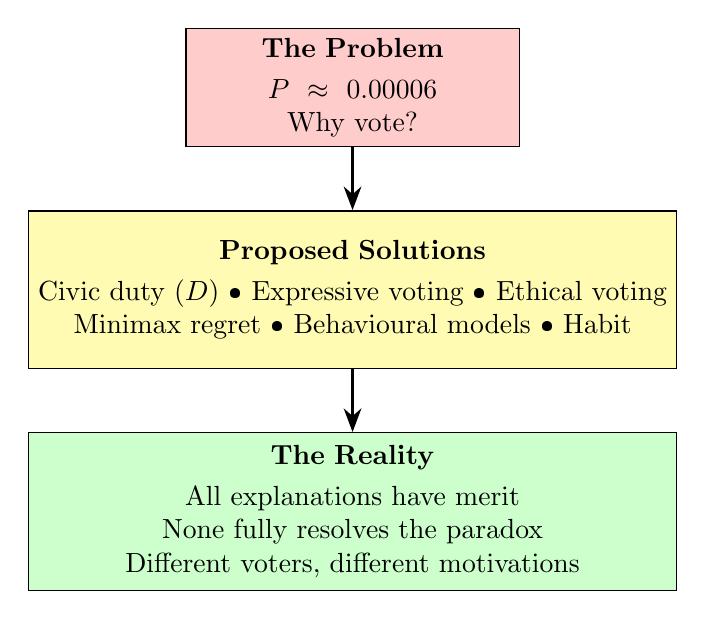
\begin{tikzpicture}[
node distance=0.8cm and 0cm, 
every node/.style={align=center, draw, rectangle, line width=0.5pt},
arrow/.style={-{Stealth[length=3mm]}, thick}
]

\node[fill=red!20, text width=4cm, minimum height=1.5cm] (problem) 
{\textbf{The Problem}\\[0.1cm] $P \approx 0.00006$\\Why vote?};


\node[fill=yellow!30, text width=8cm, minimum height=2cm, below=of problem] (solutions)
{\textbf{Proposed Solutions}\\[0.1cm]
Civic duty ($D$) \textbullet{} Expressive voting \textbullet{} Ethical voting\\
Minimax regret \textbullet{} Behavioural models \textbullet{} Habit};


\node[fill=green!20, text width=8cm, minimum height=2cm, below=of solutions] (reality)
{\textbf{The Reality}\\[0.1cm]
All explanations have merit\\
None fully resolves the paradox\\
Different voters, different motivations};


\draw[arrow] (problem) -- (solutions);
\draw[arrow] (solutions) -- (reality);

\end{tikzpicture}
\end{center}
\end{frame}


\begin{frame}{Summary: Key Takeaways}
\begin{center}
\Large \textbf{Three Things to Remember}
\end{center}

\begin{enumerate}
\item \textbf{The Math Says Don't Vote}
\begin{itemize}
\item $R = PB - C$ predicts zero turnout
\item Your vote has $\sim$6 in 100,000 chance of mattering
\end{itemize}

\vspace{0.5cm}

\item \textbf{People Vote Anyway}
\begin{itemize}
\item 50--70\% turnout in democracies worldwide
\item Not explained by pivotality ($P$)
\item Better explained by duty ($D$), expression, ethics
\end{itemize}

\vspace{0.5cm}

\item \textbf{This Matters for Democracy}
\begin{itemize}
\item Reveals limits of pure rational choice theory
\item Humans are more than selfish calculators
\item Quality of democracy depends on \emph{why} people vote
\end{itemize}
\end{enumerate}
\end{frame}

\begin{frame}[standout]
Questions?
\end{frame}


\section{Irish Context \& Applications}

\begin{frame}{Ireland's High Turnout: The Puzzle}
\textbf{Comparative perspective:}
\begin{itemize}
\item Irish general election turnout: typically 60--65\%
\item Relatively high compared to US ($\sim$55--60\%), UK ($\sim$60--70\%)
\item But lower than some European countries (Belgium 90\%+, Sweden 80\%+)
\end{itemize}



\textbf{Questions to consider:}
\begin{enumerate}
\item Does rational choice (Downsian model) explain Irish turnout?
\item Or do we need expressive/ethical voting models?
\item What Irish-specific factors might matter?
\begin{itemize}
\item PR-STV electoral system
\item Small constituencies (perception of $P$?)
\item Strong party identification
\item Political culture and civic duty
\end{itemize}
\end{enumerate}
\end{frame}

\begin{frame}{PR-STV and Voter Information Costs}
\textbf{Is PR-STV "too expensive" for the Rational Voter?}
\begin{itemize}
\item \textbf{High Information Costs ($C$):} Voters must rank multiple candidates, often from the same party.
\item \textbf{Intra-party Competition:} Differentiating between two candidates from the same party requires high "disciplined effort".
\item \textbf{Rational Ignorance:} To minimize $C$, voters may use "donkey voting" (ranking 1, 2, 3 in ballot order).
\end{itemize}



\alert{Question:} Does the complexity of PR-STV discourage marginal voters, or does it increase $B$ by giving them more choice?
\end{frame}

\begin{frame}{The "Brokerage" Effect}
\textbf{Mueller's Behavioural Model in Ireland:}
\begin{itemize}
\item \textbf{Personalized $B$:} TDs focus on local favours to provide a direct, unmistakable link to the voter's private concerns.
\item \textbf{Reinforcement:} Securing a medical card or a local road repair acts as a "token reinforcer".
\item \textbf{Result:} High turnout in rural areas may be driven by these direct "rewards" for the act of voting.
\end{itemize}



\alert{Connection to theory:} This increases the perceived $B$ (benefit) and provides behavioural reinforcement, both of which increase turnout.
\end{frame}

\begin{frame}{Irish Referendums vs. General Elections}
\textbf{Typical pattern:}
\begin{itemize}
\item Referendum turnout often \alert{lower} than general elections
\item Examples: Marriage equality (60.5\%), Lisbon Treaty (53\%, then 59\%)
\item But some referendums had high turnout (Abortion 2018: 64.1\%)
\end{itemize}



\textbf{What does Public Choice predict?}

\textbf{Argument 1: Referendums should have \emph{higher} turnout}
\begin{itemize}
\item Direct policy choice $\rightarrow$ higher $B$
\item Your vote directly determines outcome, not just who decides
\end{itemize}

\textbf{Argument 2: Referendums should have \emph{lower} turnout}
\begin{itemize}
\item No party labels to guide $\rightarrow$ higher information costs
\item Rational ignorance kicks in
\item Lower $D$ if civic duty tied to electoral cycle
\end{itemize}



Which argument is stronger? What does Irish data show?
\end{frame}

\begin{frame}{Information \& The Swing Voter's Curse}
\textbf{Feddersen \& Pesendorfer (1996): Why uncertainty leads to abstention.}

\begin{itemize}
\item \textbf{Rational Abstention:} If you don't know which candidate is better, the rational choice is to stay home to let the \emph{informed} decide.
\item \textbf{The Curse:} If an uninformed person votes, they risk "canceling out" the vote of someone who actually knows the policy details.
\item \textbf{Mueller's View:} If the reason for abstention is uncertainty, forcing people to vote (compulsory voting) is likely to \alert{worsen} democratic outcomes.
\end{itemize}



\footnotesize{Feddersen \& Pesendorfer (1996), "The Swing Voter's Curse," \emph{American Economic Review}.}
\end{frame}

\begin{frame}{Compulsory Voting for Ireland?}
\textbf{The proposal:}
\begin{itemize}
\item Small fine (€50--€100) for not voting $\rightarrow$ works in Australia, Belgium $\rightarrow$ could increase turnout to 90\%+
\end{itemize}



\textbf{Arguments in favour:}
\begin{itemize}
\item Higher participation = more legitimate outcomes
\item Forces citizens to engage with politics
\item Reduces class bias in turnout
\end{itemize}



\textbf{Public Choice counterarguments:}
\begin{itemize}
\item Brings \alert{low-$D$, uncertain} voters to polls
\item These are exactly the voters who would have abstained
\item High civic duty voters already voting
\item May \emph{reduce} quality of electoral outcomes
\item Matsusaka (1995): Uncertainty makes voting worse, not better
\end{itemize}

\alert{Key insight:} High turnout $\neq$ better democracy if marginal voters are uninformed
\end{frame}

\begin{frame}{Your Irish Context Presentations}
\textbf{Week 3 Presentation Topics:}



\textbf{Example prompts you might receive:}
\begin{itemize}
\item Why is voter turnout in Irish general elections relatively high compared to many OECD countries? Does rational choice explain this, or do we need expressive/ethical voting models?

\item Compare turnout in Irish referendums vs. general elections. What does Public Choice predict, and does the data fit?

\item Does compulsory voting (hypothetical) make sense for Ireland given the paradox of voting?
\end{itemize}



\textbf{What you're being tested on:}
\begin{itemize}
\item Understanding of rational ignorance
\item Expressive voting vs. instrumental voting
\item Role of civic duty ($D$)
\item How institutional context affects $P$, $B$, $C$, $D$
\end{itemize}
\end{frame}

\begin{frame}{Preparing Your Irish Context Presentation}
\textbf{Steps to prepare:}



\begin{enumerate}
\item \textbf{Get the data}
\begin{itemize}
\item Irish election turnout over time
\item Comparative OECD data
\item Referendum vs. election turnout
\end{itemize}

\item \textbf{Apply the theory}
\begin{itemize}
\item Does Downsian model ($R = PB - C$) explain patterns?
\item What about $R = PB + D - C$?
\item Do you need expressive/ethical models?
\end{itemize}

\item \textbf{Consider Irish-specific factors}
\begin{itemize}
\item PR-STV vs. FPTP (affects perception of $P$?)
\item Constituency size (small $\rightarrow$ higher $P$?)
\item Political culture (strong civic duty tradition?)
\end{itemize}

\item \textbf{Synthesize}
\begin{itemize}
\item Which theory best explains Irish patterns?
\item Where do the data not fit?
\end{itemize}
\end{enumerate}
\end{frame}

\begin{frame}{Hints for Irish Context Analysis}
\textbf{Useful comparisons:}
\begin{itemize}
\item Ireland vs. UK (similar culture, different electoral systems)
\item Ireland vs. Northern Ireland (same island, different contexts)
\item Ireland vs. Belgium/Australia (compulsory voting counterfactual)
\item Over-time trends in Ireland (declining or stable?)
\end{itemize}



\textbf{Key variables to consider:}
\begin{itemize}
\item Electoral system (PR-STV)
\item Constituency size (3--5 seats typical)
\item Party system (multi-party, coalition governments)
\item Referendum frequency (constitutional amendments)
\item Registration system (automatic or not?)
\end{itemize}



\textbf{Resources:}
\begin{itemize}
\item CSO (Central Statistics Office) election data
\item OECD turnout statistics
\item Academic papers on Irish voting behaviour
\end{itemize}
\end{frame}

\section{Sources / Suggestions}

\begin{frame}{Data Sources: US Voter Turnout Statistics}
\textbf{US Census Bureau Data (2020 Presidential Election):}



\small
\begin{itemize}
\item \textbf{Main Report:} Voting and Registration in the Election of November 2020 (P20-585)
\begin{itemize}
\footnotesize
\item \url{https://www.census.gov/content/dam/Census/library/publications/2022/demo/p20-585.pdf}
\end{itemize}



\item \textbf{Press Release:} 2020 Presidential Election Voting and Registration Tables
\begin{itemize}
\footnotesize
\item \url{https://www.census.gov/newsroom/press-releases/2021/2020-presidential-election-voting-and-registration-tables-now-available.html}
\end{itemize}



\item \textbf{Historical Data:} Voting and Registration time series (1964-present)
\begin{itemize}
\footnotesize
\item \url{https://www.census.gov/topics/public-sector/voting.html}
\end{itemize}
\end{itemize}
\end{frame}

\begin{frame}{Data Sources: Irish Voter Turnout Statistics}
\textbf{Central Statistics Office \& Academic Research:}



\footnotesize
\begin{itemize}
\item \textbf{CSO (2011):} Voter Participation Module, QNHS
\begin{itemize}
\scriptsize
\item \url{https://www.cso.ie/en/qnhs/qnhsmethodology/voterregistrationandparticipationmodule/}
\end{itemize}

\item \textbf{Kavanagh, A. (Maynooth):} Electoral geography and turnout patterns
\begin{itemize}
\scriptsize
\item \url{https://www.maynoothuniversity.ie/research/spotlight-research/getting-out-vote-what-influences-voter-turnout}
\end{itemize}

\item \textbf{Oireachtas Library (2016):} Election turnout in Ireland - measurement, trends and policy
\begin{itemize}
\scriptsize
\item \url{https://data.oireachtas.ie/ie/oireachtas/libraryResearch/2016/2016-01-28_l-rs-note-election-turnout-in-ireland-measurement-trends-and-policy-implications_en.pdf}
\end{itemize}

\item \textbf{RTÉ (2024):} Poll of Polls and voter turnout analysis
\begin{itemize}
\scriptsize
\item \url{https://www.rte.ie/news/election-24/2024/1124/1482646-poll-of-polls/}
\end{itemize}
\end{itemize}
\end{frame}

\begin{frame}{Further Reading: Foundational Works (Pre-1960)}
\footnotesize
\begin{enumerate}
\item Schumpeter, J. A. (1942). \emph{Capitalism, Socialism and Democracy}. New York: Harper \& Brothers.
\item Black, D. (1948). "On the Rationale of Group Decision-making." \emph{Journal of Political Economy}, 56(1), 23-34.
\item Arrow, K. J. (1951). \emph{Social Choice and Individual Values}. New York: Wiley.
\item Harsanyi, J. C. (1955). "Cardinal Welfare, Individualistic Ethics, and Interpersonal Comparisons of Utility." \emph{Journal of Political Economy}, 63(4), 309-321.
\item Downs, A. (1957). \emph{An Economic Theory of Democracy}. New York: Harper \& Row.
\end{enumerate}
\end{frame}

\begin{frame}{Further Reading: The Golden Age (1960s-1970s) — Part 1}
\footnotesize
\begin{enumerate}
\setcounter{enumi}{5}
\item Olson, M. (1965). \emph{The Logic of Collective Action}. Cambridge, MA: Harvard University Press.
\item Tullock, G. (1967). \emph{Toward a Mathematics of Politics}. Ann Arbor: University of Michigan Press.
\item Riker, W. H., \& Ordeshook, P. C. (1968). "A Theory of the Calculus of Voting." \emph{APSR}, 62(1), 25-42.
\item Riker, W. H., \& Ordeshook, P. C. (1973). \emph{An Introduction to Positive Political Theory}. Englewood Cliffs, NJ: Prentice-Hall.
\item Brody, R. A., \& Page, B. I. (1973). "Indifference, Alienation and Rational Decisions." \emph{Public Choice}, 15(1), 1-17.
\item Silver, M. (1973). "A Demand Analysis of Voting Costs and Voting Participation." \emph{Social Science Research}, 2(2), 111-124.
\end{enumerate}
\end{frame}

\begin{frame}{Further Reading: The Golden Age (1960s-1970s) — Part 2}
\footnotesize
\begin{enumerate}
\setcounter{enumi}{11}
\item Ferejohn, J. A., \& Fiorina, M. P. (1974). "The Paradox of Not Voting." \emph{APSR}, 68(2), 525-536.
\item Ferejohn, J. A., \& Fiorina, M. P. (1975). "Closeness Counts Only in Horseshoes and Dancing." \emph{APSR}, 69(3), 920-925.
\item Ashenfelter, O., \& Kelley, S., Jr. (1975). "Determinants of Participation in Presidential Elections." \emph{Journal of Law and Economics}, 18(3), 695-733.
\item Smith, J. (1975). [Oregon tax study - cited in Mueller (2003), p. 323]
\item Fiorina, M. P. (1976). "The Voting Decision: Instrumental and Expressive Aspects." \emph{Journal of Politics}, 38(2), 390-413.
\end{enumerate}
\end{frame}

\begin{frame}{Further Reading: The Golden Age (1960s-1970s) — Part 3}
\footnotesize
\begin{enumerate}
\setcounter{enumi}{16}
\item Levine, M. E., \& Plott, C. R. (1977). "Agenda Influence and Its Implications." \emph{Virginia Law Review}, 63(4), 561-604.
\item Frohlich, N., et al. (1978). "A Test of Downsian Voter Rationality: 1964 Presidential Voting." \emph{APSR}, 72(1), 178-197.
\item Kunreuther, H., et al. (1978). \emph{Disaster Insurance Protection: Public Policy Lessons}. New York: Wiley.
\item Kinder, D. R., \& Kiewiet, D. R. (1979). "Economic Discontent and Political Behaviour." \emph{American Journal of Political Science}, 23(3), 495-527.
\item Sears, D. O., et al. (1979). "Whites' Opposition to 'Busing'." \emph{APSR}, 73(2), 369-384.
\item Sears, D. O., et al. (1980). "Self-Interest vs. Symbolic Politics." \emph{APSR}, 74(3), 670-684.
\end{enumerate}
\end{frame}

\begin{frame}{Further Reading: Developments (1981-1999) — Part 1}
\footnotesize
\begin{enumerate}
\setcounter{enumi}{22}
\item Ledyard, J. O. (1981). "The Paradox of Voting and Candidate Competition." In Horwich \& Quirk (Eds.), \emph{Essays in Contemporary Fields of Economics}.
\item Marwell, G., \& Ames, R. E. (1981). "Economists Free Ride, Does Anyone Else?" \emph{Journal of Public Economics}, 15(3), 295-310.
\item Abramson, P. R., \& Aldrich, J. H. (1982). "The Decline of Electoral Participation." \emph{APSR}, 76(3), 502-521.
\item Gramlich, E. M., \& Rubinfeld, D. L. (1982). "Voting on Public Spending." \emph{Journal of Policy Analysis and Management}, 1(4), 516-533.
\item Palfrey, T. R., \& Rosenthal, H. (1983). "A Strategic Calculus of Voting." \emph{Public Choice}, 41(1), 7-53.
\item Patterson, S. C., \& Caldeira, G. A. (1983). "Getting Out the Vote." \emph{APSR}, 77(3), 675-689.
\end{enumerate}
\end{frame}

\begin{frame}{Further Reading: Developments (1981-1999) — Part 2}
\footnotesize
\begin{enumerate}
\setcounter{enumi}{28}
\item Chapman, R. G., \& Palda, K. S. (1983). "Electoral Turnout in Rational Voting." \emph{Journal of Consumer Research}, 9(4), 337-346.
\item Brennan, G., \& Buchanan, J. M. (1984). "Voter Choice: Evaluating Political Alternatives." \emph{American Behavioural Scientist}, 28(2), 185-201.
\item Foster, C. B. (1984). "The Performance of Rational Voter Models." \emph{APSR}, 78(3), 678-690.
\item Palfrey, T. R., \& Rosenthal, H. (1985). "Voter Participation and Strategic Uncertainty." \emph{APSR}, 79(1), 62-78.
\item Etzioni, A. (1986). "The Case for a Multiple-Utility Conception." \emph{Economics and Philosophy}, 2(2), 159-183.
\item Jackman, R. W. (1987). "Political Institutions and Voter Turnout." \emph{APSR}, 81(2), 405-423.
\end{enumerate}
\end{frame}

\begin{frame}{Further Reading: Developments (1981-1999) — Part 3}
\footnotesize
\begin{enumerate}
\setcounter{enumi}{34}
\item Lewis-Beck, M. S. (1988). \emph{Economics and Elections: The Major Western Democracies}. Ann Arbor: University of Michigan Press.
\item Cox, G. W., \& Munger, M. C. (1989). "Closeness, Expenditures, and Turnout." \emph{APSR}, 83(1), 217-231.
\item Kenny, C., \& Rice, T. W. (1989). "Minimax Worry in the 1980 and 1984 Presidential Elections." \emph{Western Political Quarterly}, 42(3), 443-453.
\item Carter, J., \& Guerette, S. (1992). "An Experimental Study of Expressive Voting." \emph{Public Choice}, 73(3), 251-260.
\item Aldrich, J. H. (1993). "Rational Choice and Turnout." \emph{American Journal of Political Science}, 37(1), 246-278.
\item Knack, S. (1993). "Voter Participation Effects of Selecting Jurors." \emph{Journal of Law and Economics}, 36(1), 99-114.
\end{enumerate}
\end{frame}

\begin{frame}{Further Reading: Developments (1981-1999) — Part 4}
\footnotesize
\begin{enumerate}
\setcounter{enumi}{40}
\item Matsusaka, J. G., \& Palda, F. (1993). "The Downsian Voter Meets the Ecological Fallacy." \emph{Public Choice}, 77(4), 855-878.
\item Knack, S. (1994). "Does Rain Help the Republicans?" \emph{Public Choice}, 79(1-2), 187-209.
\item Hudson, J., \& Jones, P. (1994). "The Importance of Being a 'B' or 'C'." \emph{Public Choice}, 81(3-4), 313-328.
\item Blais, A., et al. (1995). "Do People Vote on the Basis of Minimax Regret?" \emph{Political Research Quarterly}, 48(4), 827-836.
\item Heckelman, J. C. (1995). "The Effect of the Secret Ballot." \emph{Public Choice}, 82(1-2), 107-124.
\item Matsusaka, J. G. (1995). "Explaining Voter Turnout Patterns." \emph{Public Choice}, 84(1-2), 91-117.
\end{enumerate}
\end{frame}

\begin{frame}{Further Reading: Developments (1981-1999) — Part 5}
\footnotesize
\begin{enumerate}
\setcounter{enumi}{46}
\item Feddersen, T. J., \& Pesendorfer, W. (1996). "The Swing Voter's Curse." \emph{American Economic Review}, 86(3), 408-424.
\item Fischer, A. J. (1996). "A Further Experimental Study of Expressive Voting." \emph{Public Choice}, 88(1-2), 171-184.
\item Nannestad, P., \& Paldam, M. (1996). "The VP-Function." \emph{Public Choice}, 79(3-4), 213-245.
\item Aldrich, J. H. (1997). "When Is It Rational to Vote?" In Mueller (Ed.), \emph{Perspectives on Public Choice}.
\item Cox, G. W. (1997). \emph{Making Votes Count}. Cambridge: Cambridge University Press.
\item Fiorina, M. P. (1997). "Voting Behaviour." In Mueller (Ed.), \emph{Perspectives on Public Choice}.
\end{enumerate}
\end{frame}

\begin{frame}{Further Reading: Developments (1981-1999) — Part 6}
\footnotesize
\begin{enumerate}
\setcounter{enumi}{52}
\item Nannestad, P., \& Paldam, M. (1997). "From the Pocketbook of the Welfare State." \emph{European Journal of Political Research}, 31(1), 109-136.
\item Blais, A., \& Young, R. (1999). "Why Do People Vote? An Experiment in Rationality." \emph{Public Choice}, 99(1-2), 39-55.
\item Matsusaka, J. G., \& Palda, F. (1999). "Voter Turnout: How Much Can We Explain?" \emph{Public Choice}, 98(3-4), 431-446.
\item Shachar, R., \& Nalebuff, B. (1999). "Follow the Leader." \emph{American Economic Review}, 89(3), 525-547.
\end{enumerate}
\end{frame}

\begin{frame}{Further Reading: Modern Works (2000-Present)}
\footnotesize
\begin{enumerate}
\setcounter{enumi}{56}
\item Heckelman, J. C. (2000). "The Secret Ballot and the Realignment of 1892." \emph{Social Science History}, 24(3), 567-591.
\item Knack, S. (2000). "Deterring Voter Registration Through Juror Selection." \emph{Public Choice}, 103(1-2), 49-62.
\item Mueller, D. C. (2003). \emph{Public Choice III}. Cambridge: Cambridge University Press. [Chapter 14]
\item Feddersen, T. J. (2004). "Rational Choice Theory and the Paradox of Not Voting." \emph{Journal of Economic Perspectives}, 18(1), 99-112.
\item Gerber, A. S., et al. (2008). "Social Pressure and Voter Turnout." \emph{APSR}, 102(1), 33-48.
\item DellaVigna, S., et al. (2017). "Voting to Tell Others." \emph{Review of Economic Studies}, 84(1), 143-181.
\end{enumerate}
\end{frame}

\begin{frame}{Cultural Resources: Films \& TV Series}
\textbf{Strategic Political Behaviour \& Cynicism:}
\begin{itemize}
\item \textbf{House of Cards} (USA, Season 1) - Strategic manipulation and rational self-interest
\item \textbf{Veep} - Satirical take on political motivations
\item \textbf{The Thick of It} (UK) - Cynical comedy about political spin
\end{itemize}



\textbf{Civic Duty \& Idealism (the counterpoint):}
\begin{itemize}
\item \textbf{The West Wing} - Public service as noble calling
\item \textbf{Parks and Recreation} - Local government and civic engagement
\item \textbf{Mr. Smith Goes to Washington} (1939) - Classic civic duty ideal
\end{itemize}



\textbf{Social Media \& Political Performance:}
\begin{itemize}
\item \textbf{The Social Dilemma} (Netflix) - Connects to our social media discussion
\end{itemize}
\end{frame}

\begin{frame}{Cultural Resources: Books \& Essays}
\textbf{Directly relevant to this lecture:}
\begin{itemize}
\item Bryan Caplan - \emph{The Myth of the Rational Voter} (2007)
\item Nassim Taleb - "The Most Intolerant Wins: The Dictatorship of the Small Minority"
\item Mancur Olson - \emph{The Logic of Collective Action} (already in your reading list!)
\end{itemize}



\textbf{For Irish Context:}
\begin{itemize}
\item \textbf{Reeling in the Years} (RTÉ) - Irish political/cultural history
\item Episodes covering referendum campaigns (divorce, abortion, marriage equality)
\end{itemize}



\textbf{Podcasts:}
\begin{itemize}
\item \textbf{EconTalk} - Episodes with Michael Munger, Bryan Caplan on voting
\item \textbf{More or Less} (BBC) - Statistical literacy in politics
\item \textbf{Good on Paper} - "Did Busing Turn Kids Into Democrats?" (Episode on how school integration shaped political identities)
\end{itemize}
\end{frame}

\begin{frame}{How to Engage with These Resources}
\textbf{Suggested approach:}
\begin{enumerate}
\item Pick one that interests you
\item Watch/read with the lecture models in mind
\item Ask yourself:
\begin{itemize}
\item Are characters motivated by $PB$, $D$, expressive benefits, or ethical concerns?
\item Do they behave as rational actors?
\item Where does the model break down?
\end{itemize}
\item Consider discussing in your Irish Context presentations
\end{enumerate}



\alert{Remember:} These are cultural representations and not rigorous analysis - but they can help you think critically about political behaviour models!
\end{frame}

\end{document}